\documentclass[1p]{elsarticle_modified}
%\bibliographystyle{elsarticle-num}

%\usepackage[colorlinks]{hyperref}
%\usepackage{abbrmath_seonhwa} %\Abb, \Ascr, \Acal ,\Abf, \Afrak
\usepackage{amsfonts}
\usepackage{amssymb}
\usepackage{amsmath}
\usepackage{amsthm}
\usepackage{scalefnt}
\usepackage{amsbsy}
\usepackage{kotex}
\usepackage{caption}
\usepackage{subfig}
\usepackage{color}
\usepackage{graphicx}
\usepackage{xcolor} %% white, black, red, green, blue, cyan, magenta, yellow
\usepackage{float}
\usepackage{setspace}
\usepackage{hyperref}

\usepackage{tikz}
\usetikzlibrary{arrows}

\usepackage{multirow}
\usepackage{array} % fixed length table
\usepackage{hhline}

%%%%%%%%%%%%%%%%%%%%%
\makeatletter
\renewcommand*\env@matrix[1][\arraystretch]{%
	\edef\arraystretch{#1}%
	\hskip -\arraycolsep
	\let\@ifnextchar\new@ifnextchar
	\array{*\c@MaxMatrixCols c}}
\makeatother %https://tex.stackexchange.com/questions/14071/how-can-i-increase-the-line-spacing-in-a-matrix
%%%%%%%%%%%%%%%

\usepackage[normalem]{ulem}

\newcommand{\msout}[1]{\ifmmode\text{\sout{\ensuremath{#1}}}\else\sout{#1}\fi}
%SOURCE: \msout is \stkout macro in https://tex.stackexchange.com/questions/20609/strikeout-in-math-mode

\newcommand{\cancel}[1]{
	\ifmmode
	{\color{red}\msout{#1}}
	\else
	{\color{red}\sout{#1}}
	\fi
}

\newcommand{\add}[1]{
	{\color{blue}\uwave{#1}}
}

\newcommand{\replace}[2]{
	\ifmmode
	{\color{red}\msout{#1}}{\color{blue}\uwave{#2}}
	\else
	{\color{red}\sout{#1}}{\color{blue}\uwave{#2}}
	\fi
}

\newcommand{\Sol}{\mathcal{S}} %segment
\newcommand{\D}{D} %diagram
\newcommand{\A}{\mathcal{A}} %arc


%%%%%%%%%%%%%%%%%%%%%%%%%%%%%5 test

\def\sl{\operatorname{\textup{SL}}(2,\Cbb)}
\def\psl{\operatorname{\textup{PSL}}(2,\Cbb)}
\def\quan{\mkern 1mu \triangleright \mkern 1mu}

\theoremstyle{definition}
\newtheorem{thm}{Theorem}[section]
\newtheorem{prop}[thm]{Proposition}
\newtheorem{lem}[thm]{Lemma}
\newtheorem{ques}[thm]{Question}
\newtheorem{cor}[thm]{Corollary}
\newtheorem{defn}[thm]{Definition}
\newtheorem{exam}[thm]{Example}
\newtheorem{rmk}[thm]{Remark}
\newtheorem{alg}[thm]{Algorithm}

\newcommand{\I}{\sqrt{-1}}
\begin{document}

%\begin{frontmatter}
%
%\title{Boundary parabolic representations of knots up to 8 crossings}
%
%%% Group authors per affiliation:
%\author{Yunhi Cho} 
%\address{Department of Mathematics, University of Seoul, Seoul, Korea}
%\ead{yhcho@uos.ac.kr}
%
%
%\author{Seonhwa Kim} %\fnref{s_kim}}
%\address{Center for Geometry and Physics, Institute for Basic Science, Pohang, 37673, Korea}
%\ead{ryeona17@ibs.re.kr}
%
%\author{Hyuk Kim}
%\address{Department of Mathematical Sciences, Seoul National University, Seoul 08826, Korea}
%\ead{hyukkim@snu.ac.kr}
%
%\author{Seokbeom Yoon}
%\address{Department of Mathematical Sciences, Seoul National University, Seoul, 08826,  Korea}
%\ead{sbyoon15@snu.ac.kr}
%
%\begin{abstract}
%We find all boundary parabolic representation of knots up to 8 crossings.
%
%\end{abstract}
%\begin{keyword}
%    \MSC[2010] 57M25 
%\end{keyword}
%
%\end{frontmatter}

%\linenumbers
%\tableofcontents
%
\newcommand\colored[1]{\textcolor{white}{\rule[-0.35ex]{0.8em}{1.4ex}}\kern-0.8em\color{red} #1}%
%\newcommand\colored[1]{\textcolor{white}{ #1}\kern-2.17ex	\textcolor{white}{ #1}\kern-1.81ex	\textcolor{white}{ #1}\kern-2.15ex\color{red}#1	}

{\Large $\underline{12a_{1255}~(K12a_{1255})}$}

\setlength{\tabcolsep}{10pt}
\renewcommand{\arraystretch}{1.6}
\vspace{1cm}\begin{tabular}{m{100pt}>{\centering\arraybackslash}m{274pt}}
\multirow{5}{120pt}{
	\centering
	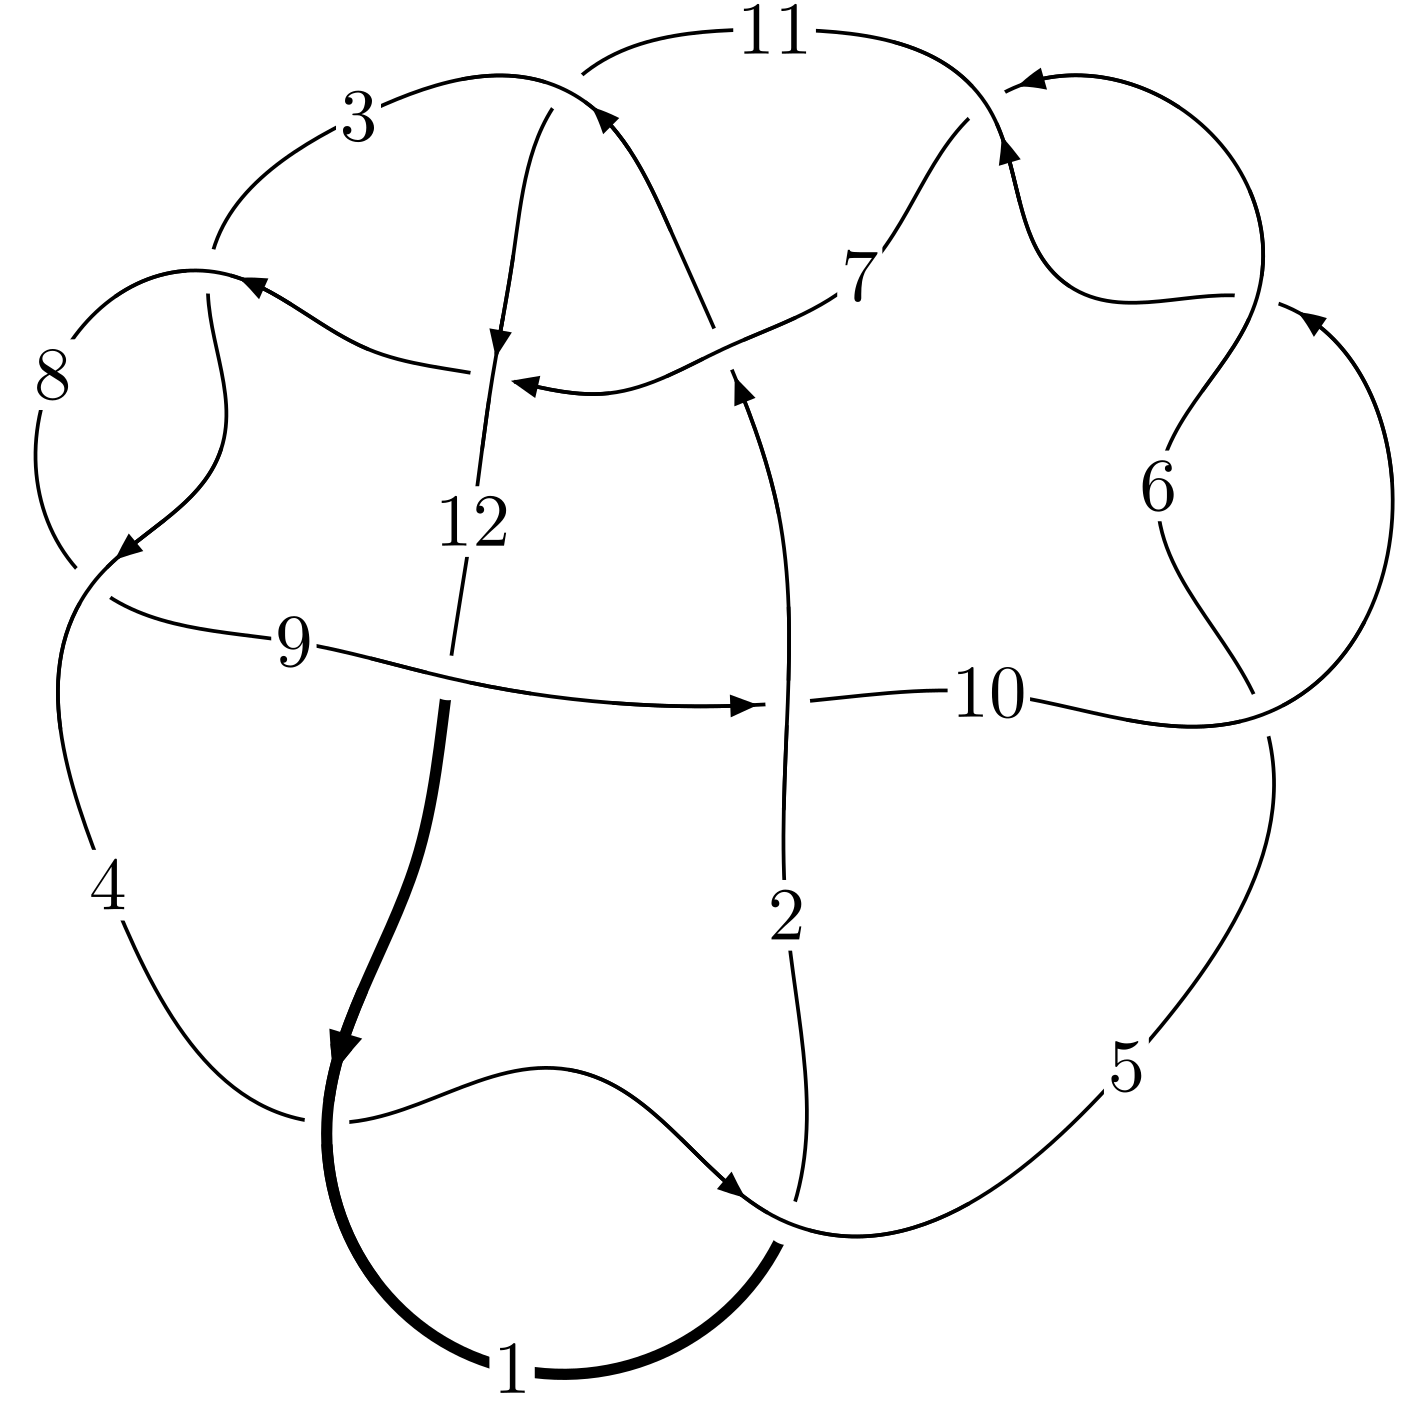
\includegraphics[width=112pt]{../../../GIT/diagram.site/Diagrams/png/2056_12a_1255.png}\\
\ \ \ A knot diagram\footnotemark}&
\allowdisplaybreaks
\textbf{Linearized knot diagam} \\
\cline{2-2}
 &
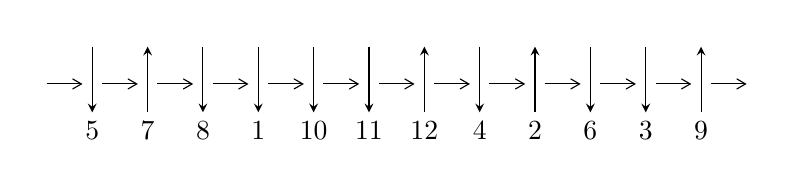
\begin{tikzpicture}[x=20pt, y=17pt]
	% nodes
	\node (C0) at (0, 0) {};
	\node (C1) at (1, 0) {};
	\node (C1U) at (1, +1) {};
	\node (C1D) at (1, -1) {5};

	\node (C2) at (2, 0) {};
	\node (C2U) at (2, +1) {};
	\node (C2D) at (2, -1) {7};

	\node (C3) at (3, 0) {};
	\node (C3U) at (3, +1) {};
	\node (C3D) at (3, -1) {8};

	\node (C4) at (4, 0) {};
	\node (C4U) at (4, +1) {};
	\node (C4D) at (4, -1) {1};

	\node (C5) at (5, 0) {};
	\node (C5U) at (5, +1) {};
	\node (C5D) at (5, -1) {10};

	\node (C6) at (6, 0) {};
	\node (C6U) at (6, +1) {};
	\node (C6D) at (6, -1) {11};

	\node (C7) at (7, 0) {};
	\node (C7U) at (7, +1) {};
	\node (C7D) at (7, -1) {12};

	\node (C8) at (8, 0) {};
	\node (C8U) at (8, +1) {};
	\node (C8D) at (8, -1) {4};

	\node (C9) at (9, 0) {};
	\node (C9U) at (9, +1) {};
	\node (C9D) at (9, -1) {2};

	\node (C10) at (10, 0) {};
	\node (C10U) at (10, +1) {};
	\node (C10D) at (10, -1) {6};

	\node (C11) at (11, 0) {};
	\node (C11U) at (11, +1) {};
	\node (C11D) at (11, -1) {3};

	\node (C12) at (12, 0) {};
	\node (C12U) at (12, +1) {};
	\node (C12D) at (12, -1) {9};
	\node (C13) at (13, 0) {};

	% arrows
	\draw[->,>={angle 60}]
	(C0) edge (C1) (C1) edge (C2) (C2) edge (C3) (C3) edge (C4) (C4) edge (C5) (C5) edge (C6) (C6) edge (C7) (C7) edge (C8) (C8) edge (C9) (C9) edge (C10) (C10) edge (C11) (C11) edge (C12) (C12) edge (C13) ;	\draw[->,>=stealth]
	(C1U) edge (C1D) (C2D) edge (C2U) (C3U) edge (C3D) (C4U) edge (C4D) (C5U) edge (C5D) (C6U) edge (C6D) (C7D) edge (C7U) (C8U) edge (C8D) (C9D) edge (C9U) (C10U) edge (C10D) (C11U) edge (C11D) (C12D) edge (C12U) ;
	\end{tikzpicture} \\
\hhline{~~} \\& 
\textbf{Solving Sequence} \\ \cline{2-2} 
 &
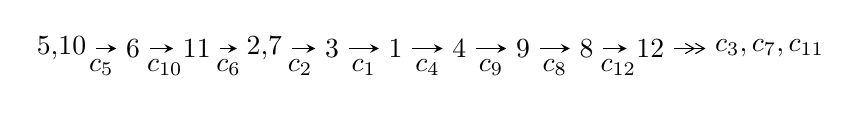
\begin{tikzpicture}[x=23pt, y=7pt]
	% node
	\node (A0) at (-1/8, 0) {5,10};
	\node (A1) at (1, 0) {6};
	\node (A2) at (2, 0) {11};
	\node (A3) at (49/16, 0) {2,7};
	\node (A4) at (33/8, 0) {3};
	\node (A5) at (41/8, 0) {1};
	\node (A6) at (49/8, 0) {4};
	\node (A7) at (57/8, 0) {9};
	\node (A8) at (65/8, 0) {8};
	\node (A9) at (73/8, 0) {12};
	\node (C1) at (1/2, -1) {$c_{5}$};
	\node (C2) at (3/2, -1) {$c_{10}$};
	\node (C3) at (5/2, -1) {$c_{6}$};
	\node (C4) at (29/8, -1) {$c_{2}$};
	\node (C5) at (37/8, -1) {$c_{1}$};
	\node (C6) at (45/8, -1) {$c_{4}$};
	\node (C7) at (53/8, -1) {$c_{9}$};
	\node (C8) at (61/8, -1) {$c_{8}$};
	\node (C9) at (69/8, -1) {$c_{12}$};
	\node (A10) at (11, 0) {$c_{3},c_{7},c_{11}$};

	% edge
	\draw[->,>=stealth]	
	(A0) edge (A1) (A1) edge (A2) (A2) edge (A3) (A3) edge (A4) (A4) edge (A5) (A5) edge (A6) (A6) edge (A7) (A7) edge (A8) (A8) edge (A9) ;
	\draw[->>,>={angle 60}]	
	(A9) edge (A10);
\end{tikzpicture} \\ 

\end{tabular} \\

\footnotetext{
The image of knot diagram is generated by the software ``\textbf{Draw programme}" developed by Andrew Bartholomew(\url{http://www.layer8.co.uk/maths/draw/index.htm\#Running-draw}), where we modified some parts for our purpose(\url{https://github.com/CATsTAILs/LinksPainter}).
}\phantom \\ \newline 
\centering \textbf{Ideals for irreducible components\footnotemark of $X_{\text{par}}$} 
 
\begin{align*}
I^u_{1}&=\langle 
2.19271\times10^{265} u^{102}+5.65299\times10^{265} u^{101}+\cdots+3.59709\times10^{264} b-5.56869\times10^{266},\\
\phantom{I^u_{1}}&\phantom{= \langle  }3.41923\times10^{266} u^{102}+8.30043\times10^{266} u^{101}+\cdots+7.91361\times10^{265} a-4.72551\times10^{267},\\
\phantom{I^u_{1}}&\phantom{= \langle  }u^{103}+3 u^{102}+\cdots-30 u-11\rangle \\
I^u_{2}&=\langle 
u^{13}+2 u^{12}-8 u^{11}-14 u^{10}+25 u^9+35 u^8-31 u^7-32 u^6- u^5-3 u^4+24 u^3+18 u^2+b-3 u-2,\\
\phantom{I^u_{2}}&\phantom{= \langle  }-6 u^{13}-9 u^{12}+\cdots+a+17,\\
\phantom{I^u_{2}}&\phantom{= \langle  }u^{14}+u^{13}-9 u^{12}-7 u^{11}+30 u^{10}+18 u^9-41 u^8-19 u^7+10 u^6+3 u^5+21 u^4+7 u^3-10 u^2- u+1\rangle \\
I^u_{3}&=\langle 
b+1,\;a^2+a-1,\;u-1\rangle \\
I^u_{4}&=\langle 
b,\;a+1,\;u-1\rangle \\
\\
\end{align*}
\raggedright * 4 irreducible components of $\dim_{\mathbb{C}}=0$, with total 120 representations.\\
\footnotetext{All coefficients of polynomials are rational numbers. But the coefficients are sometimes approximated in decimal forms when there is not enough margin.}
\newpage
\renewcommand{\arraystretch}{1}
\centering \section*{I. $I^u_{1}= \langle 2.19\times10^{265} u^{102}+5.65\times10^{265} u^{101}+\cdots+3.60\times10^{264} b-5.57\times10^{266},\;3.42\times10^{266} u^{102}+8.30\times10^{266} u^{101}+\cdots+7.91\times10^{265} a-4.73\times10^{267},\;u^{103}+3 u^{102}+\cdots-30 u-11 \rangle$}
\flushleft \textbf{(i) Arc colorings}\\
\begin{tabular}{m{7pt} m{180pt} m{7pt} m{180pt} }
\flushright $a_{5}=$&$\begin{pmatrix}1\\0\end{pmatrix}$ \\
\flushright $a_{10}=$&$\begin{pmatrix}0\\u\end{pmatrix}$ \\
\flushright $a_{6}=$&$\begin{pmatrix}1\\u^2\end{pmatrix}$ \\
\flushright $a_{11}=$&$\begin{pmatrix}- u\\- u^3+u\end{pmatrix}$ \\
\flushright $a_{2}=$&$\begin{pmatrix}-4.32069 u^{102}-10.4888 u^{101}+\cdots+179.840 u+59.7137\\-6.09577 u^{102}-15.7154 u^{101}+\cdots+63.8206 u+154.811\end{pmatrix}$ \\
\flushright $a_{7}=$&$\begin{pmatrix}- u^2+1\\- u^4+2 u^2\end{pmatrix}$ \\
\flushright $a_{3}=$&$\begin{pmatrix}-6.71410 u^{102}-16.7635 u^{101}+\cdots+184.719 u+127.421\\-6.80402 u^{102}-17.5816 u^{101}+\cdots+64.6779 u+175.953\end{pmatrix}$ \\
\flushright $a_{1}=$&$\begin{pmatrix}-10.4165 u^{102}-26.2042 u^{101}+\cdots+243.661 u+214.524\\-6.09577 u^{102}-15.7154 u^{101}+\cdots+63.8206 u+154.811\end{pmatrix}$ \\
\flushright $a_{4}=$&$\begin{pmatrix}-9.75655 u^{102}-25.0868 u^{101}+\cdots+64.3501 u+243.568\\0.623874 u^{102}+1.58451 u^{101}+\cdots-20.0995 u-19.7696\end{pmatrix}$ \\
\flushright $a_{9}=$&$\begin{pmatrix}-4.30255 u^{102}-11.7953 u^{101}+\cdots-115.645 u+167.369\\4.46999 u^{102}+11.4379 u^{101}+\cdots-48.0748 u-114.185\end{pmatrix}$ \\
\flushright $a_{8}=$&$\begin{pmatrix}-14.1641 u^{102}-36.5893 u^{101}+\cdots+32.7208 u+379.312\\-0.623051 u^{102}-1.57175 u^{101}+\cdots+2.42488 u+11.4572\end{pmatrix}$ \\
\flushright $a_{12}=$&$\begin{pmatrix}3.73375 u^{102}+9.15179 u^{101}+\cdots-141.830 u-66.2722\\1.12589 u^{102}+2.84348 u^{101}+\cdots-12.2490 u-30.2912\end{pmatrix}$\\&\end{tabular}
\flushleft \textbf{(ii) Obstruction class $= -1$}\\~\\
\flushleft \textbf{(iii) Cusp Shapes $= 8.97892 u^{102}+21.2749 u^{101}+\cdots-439.789 u-159.114$}\\~\\
\newpage\renewcommand{\arraystretch}{1}
\flushleft \textbf{(iv) u-Polynomials at the component}\newline \\
\begin{tabular}{m{50pt}|m{274pt}}
Crossings & \hspace{64pt}u-Polynomials at each crossing \\
\hline $$\begin{aligned}c_{1},c_{4}\end{aligned}$$&$\begin{aligned}
&u^{103}+5 u^{102}+\cdots-140 u-5
\end{aligned}$\\
\hline $$\begin{aligned}c_{2}\end{aligned}$$&$\begin{aligned}
&u^{103}-6 u^{102}+\cdots-2684 u-1763
\end{aligned}$\\
\hline $$\begin{aligned}c_{3},c_{8}\end{aligned}$$&$\begin{aligned}
&u^{103}-3 u^{102}+\cdots-340 u+41
\end{aligned}$\\
\hline $$\begin{aligned}c_{5},c_{6},c_{10}\end{aligned}$$&$\begin{aligned}
&u^{103}-3 u^{102}+\cdots-30 u+11
\end{aligned}$\\
\hline $$\begin{aligned}c_{7}\end{aligned}$$&$\begin{aligned}
&u^{103}-6 u^{102}+\cdots-120 u-20
\end{aligned}$\\
\hline $$\begin{aligned}c_{9}\end{aligned}$$&$\begin{aligned}
&u^{103}-4 u^{102}+\cdots-558937 u-115993
\end{aligned}$\\
\hline $$\begin{aligned}c_{11}\end{aligned}$$&$\begin{aligned}
&u^{103}+4 u^{102}+\cdots-37150 u-3953
\end{aligned}$\\
\hline $$\begin{aligned}c_{12}\end{aligned}$$&$\begin{aligned}
&u^{103}+3 u^{102}+\cdots-3395 u+319
\end{aligned}$\\
\hline
\end{tabular}\\~\\
\newpage\renewcommand{\arraystretch}{1}
\flushleft \textbf{(v) Riley Polynomials at the component}\newline \\
\begin{tabular}{m{50pt}|m{274pt}}
Crossings & \hspace{64pt}Riley Polynomials at each crossing \\
\hline $$\begin{aligned}c_{1},c_{4}\end{aligned}$$&$\begin{aligned}
&y^{103}-117 y^{102}+\cdots+2440 y-25
\end{aligned}$\\
\hline $$\begin{aligned}c_{2}\end{aligned}$$&$\begin{aligned}
&y^{103}-20 y^{102}+\cdots-30171744 y-3108169
\end{aligned}$\\
\hline $$\begin{aligned}c_{3},c_{8}\end{aligned}$$&$\begin{aligned}
&y^{103}-89 y^{102}+\cdots+19496 y-1681
\end{aligned}$\\
\hline $$\begin{aligned}c_{5},c_{6},c_{10}\end{aligned}$$&$\begin{aligned}
&y^{103}-115 y^{102}+\cdots+10294 y-121
\end{aligned}$\\
\hline $$\begin{aligned}c_{7}\end{aligned}$$&$\begin{aligned}
&y^{103}-18 y^{102}+\cdots+14360 y-400
\end{aligned}$\\
\hline $$\begin{aligned}c_{9}\end{aligned}$$&$\begin{aligned}
&y^{103}+42 y^{102}+\cdots-65353344557 y-13454376049
\end{aligned}$\\
\hline $$\begin{aligned}c_{11}\end{aligned}$$&$\begin{aligned}
&y^{103}-48 y^{102}+\cdots+1279676770 y-15626209
\end{aligned}$\\
\hline $$\begin{aligned}c_{12}\end{aligned}$$&$\begin{aligned}
&y^{103}+21 y^{102}+\cdots+6596199 y-101761
\end{aligned}$\\
\hline
\end{tabular}\\~\\
\newpage\flushleft \textbf{(vi) Complex Volumes and Cusp Shapes}
$$\begin{array}{c|c|c}  
\text{Solutions to }I^u_{1}& \I (\text{vol} + \sqrt{-1}CS) & \text{Cusp shape}\\
 \hline 
\begin{aligned}
u &= -1.02714\phantom{ +0.000000I} \\
a &= -0.871216\phantom{ +0.000000I} \\
b &= \phantom{-}1.12945\phantom{ +0.000000I}\end{aligned}
 & -2.83707\phantom{ +0.000000I} & \phantom{-0.000000 } 0 \\ \hline\begin{aligned}
u &= -0.712753 + 0.660374 I \\
a &= \phantom{-}0.12981 - 1.48426 I \\
b &= -1.243000 + 0.352054 I\end{aligned}
 & -1.53336 + 8.26614 I & \phantom{-0.000000 } 0 \\ \hline\begin{aligned}
u &= -0.712753 - 0.660374 I \\
a &= \phantom{-}0.12981 + 1.48426 I \\
b &= -1.243000 - 0.352054 I\end{aligned}
 & -1.53336 - 8.26614 I & \phantom{-0.000000 } 0 \\ \hline\begin{aligned}
u &= \phantom{-}0.571147 + 0.776168 I \\
a &= \phantom{-}0.698957 - 0.445070 I \\
b &= \phantom{-}0.043595 + 0.727181 I\end{aligned}
 & -2.06014 + 3.60547 I & \phantom{-0.000000 } 0 \\ \hline\begin{aligned}
u &= \phantom{-}0.571147 - 0.776168 I \\
a &= \phantom{-}0.698957 + 0.445070 I \\
b &= \phantom{-}0.043595 - 0.727181 I\end{aligned}
 & -2.06014 - 3.60547 I & \phantom{-0.000000 } 0 \\ \hline\begin{aligned}
u &= \phantom{-}0.922298 + 0.546376 I \\
a &= \phantom{-}0.492087 + 0.603509 I \\
b &= -1.352480 + 0.129722 I\end{aligned}
 & -6.42162 + 1.25693 I & \phantom{-0.000000 } 0 \\ \hline\begin{aligned}
u &= \phantom{-}0.922298 - 0.546376 I \\
a &= \phantom{-}0.492087 - 0.603509 I \\
b &= -1.352480 - 0.129722 I\end{aligned}
 & -6.42162 - 1.25693 I & \phantom{-0.000000 } 0 \\ \hline\begin{aligned}
u &= \phantom{-}0.696204 + 0.862353 I \\
a &= \phantom{-}0.393640 + 0.810036 I \\
b &= -1.202830 - 0.163141 I\end{aligned}
 & -3.80047 - 3.13987 I & \phantom{-0.000000 } 0 \\ \hline\begin{aligned}
u &= \phantom{-}0.696204 - 0.862353 I \\
a &= \phantom{-}0.393640 - 0.810036 I \\
b &= -1.202830 + 0.163141 I\end{aligned}
 & -3.80047 + 3.13987 I & \phantom{-0.000000 } 0 \\ \hline\begin{aligned}
u &= \phantom{-}0.519592 + 0.712577 I \\
a &= -0.036788 + 1.108860 I \\
b &= -0.297248 - 1.015470 I\end{aligned}
 & -1.98401 - 8.53931 I & \phantom{-0.000000 } 0\\
 \hline 
 \end{array}$$\newpage$$\begin{array}{c|c|c}  
\text{Solutions to }I^u_{1}& \I (\text{vol} + \sqrt{-1}CS) & \text{Cusp shape}\\
 \hline 
\begin{aligned}
u &= \phantom{-}0.519592 - 0.712577 I \\
a &= -0.036788 - 1.108860 I \\
b &= -0.297248 + 1.015470 I\end{aligned}
 & -1.98401 + 8.53931 I & \phantom{-0.000000 } 0 \\ \hline\begin{aligned}
u &= -0.263680 + 0.825383 I \\
a &= \phantom{-}0.826687 + 0.113153 I \\
b &= -1.100060 - 0.204003 I\end{aligned}
 & -0.18116 - 3.40409 I & \phantom{-0.000000 } 0 \\ \hline\begin{aligned}
u &= -0.263680 - 0.825383 I \\
a &= \phantom{-}0.826687 - 0.113153 I \\
b &= -1.100060 + 0.204003 I\end{aligned}
 & -0.18116 + 3.40409 I & \phantom{-0.000000 } 0 \\ \hline\begin{aligned}
u &= \phantom{-}0.864517 + 0.038493 I \\
a &= -0.737989 - 0.406950 I \\
b &= -1.44132 - 0.20978 I\end{aligned}
 & -6.85390 - 0.24458 I & \phantom{-0.000000 } 0 \\ \hline\begin{aligned}
u &= \phantom{-}0.864517 - 0.038493 I \\
a &= -0.737989 + 0.406950 I \\
b &= -1.44132 + 0.20978 I\end{aligned}
 & -6.85390 + 0.24458 I & \phantom{-0.000000 } 0 \\ \hline\begin{aligned}
u &= \phantom{-}0.777485 + 0.829059 I \\
a &= -0.197802 - 1.189670 I \\
b &= \phantom{-}1.42684 + 0.40686 I\end{aligned}
 & -7.3811 - 13.5504 I & \phantom{-0.000000 } 0 \\ \hline\begin{aligned}
u &= \phantom{-}0.777485 - 0.829059 I \\
a &= -0.197802 + 1.189670 I \\
b &= \phantom{-}1.42684 - 0.40686 I\end{aligned}
 & -7.3811 + 13.5504 I & \phantom{-0.000000 } 0 \\ \hline\begin{aligned}
u &= \phantom{-}0.833384\phantom{ +0.000000I} \\
a &= \phantom{-}2.76816\phantom{ +0.000000I} \\
b &= \phantom{-}1.04792\phantom{ +0.000000I}\end{aligned}
 & -3.08922\phantom{ +0.000000I} & \phantom{-0.000000 } 0 \\ \hline\begin{aligned}
u &= -0.780557 + 0.878110 I \\
a &= -0.287845 + 0.849782 I \\
b &= \phantom{-}1.36372 - 0.41744 I\end{aligned}
 & -8.07615 + 4.22446 I & \phantom{-0.000000 } 0 \\ \hline\begin{aligned}
u &= -0.780557 - 0.878110 I \\
a &= -0.287845 - 0.849782 I \\
b &= \phantom{-}1.36372 + 0.41744 I\end{aligned}
 & -8.07615 - 4.22446 I & \phantom{-0.000000 } 0\\
 \hline 
 \end{array}$$\newpage$$\begin{array}{c|c|c}  
\text{Solutions to }I^u_{1}& \I (\text{vol} + \sqrt{-1}CS) & \text{Cusp shape}\\
 \hline 
\begin{aligned}
u &= -0.629722 + 0.992893 I \\
a &= -0.637158 + 0.631730 I \\
b &= \phantom{-}1.283490 + 0.135693 I\end{aligned}
 & -7.56113 + 2.31048 I & \phantom{-0.000000 } 0 \\ \hline\begin{aligned}
u &= -0.629722 - 0.992893 I \\
a &= -0.637158 - 0.631730 I \\
b &= \phantom{-}1.283490 - 0.135693 I\end{aligned}
 & -7.56113 - 2.31048 I & \phantom{-0.000000 } 0 \\ \hline\begin{aligned}
u &= \phantom{-}0.300171 + 0.742213 I \\
a &= \phantom{-}1.20411 + 1.29920 I \\
b &= -1.366820 - 0.263059 I\end{aligned}
 & -4.56735 - 5.86087 I & \phantom{-0.000000 } 0 \\ \hline\begin{aligned}
u &= \phantom{-}0.300171 - 0.742213 I \\
a &= \phantom{-}1.20411 - 1.29920 I \\
b &= -1.366820 + 0.263059 I\end{aligned}
 & -4.56735 + 5.86087 I & \phantom{-0.000000 } 0 \\ \hline\begin{aligned}
u &= -0.524235 + 0.540945 I \\
a &= \phantom{-}0.320803 + 1.183620 I \\
b &= -0.017847 - 0.806346 I\end{aligned}
 & \phantom{-}2.26250 + 4.10162 I & \phantom{-0.000000 } 0 \\ \hline\begin{aligned}
u &= -0.524235 - 0.540945 I \\
a &= \phantom{-}0.320803 - 1.183620 I \\
b &= -0.017847 + 0.806346 I\end{aligned}
 & \phantom{-}2.26250 - 4.10162 I & \phantom{-0.000000 } 0 \\ \hline\begin{aligned}
u &= \phantom{-}0.336627 + 1.200440 I \\
a &= -0.602563 + 0.003656 I \\
b &= \phantom{-}1.278080 - 0.281645 I\end{aligned}
 & -5.92485 + 7.20612 I & \phantom{-0.000000 } 0 \\ \hline\begin{aligned}
u &= \phantom{-}0.336627 - 1.200440 I \\
a &= -0.602563 - 0.003656 I \\
b &= \phantom{-}1.278080 + 0.281645 I\end{aligned}
 & -5.92485 - 7.20612 I & \phantom{-0.000000 } 0 \\ \hline\begin{aligned}
u &= \phantom{-}0.739866 + 0.039993 I \\
a &= -1.076040 - 0.142388 I \\
b &= \phantom{-}0.274494 - 0.030365 I\end{aligned}
 & -1.57618 - 0.01678 I & \phantom{-0.000000 } 0 \\ \hline\begin{aligned}
u &= \phantom{-}0.739866 - 0.039993 I \\
a &= -1.076040 + 0.142388 I \\
b &= \phantom{-}0.274494 + 0.030365 I\end{aligned}
 & -1.57618 + 0.01678 I & \phantom{-0.000000 } 0\\
 \hline 
 \end{array}$$\newpage$$\begin{array}{c|c|c}  
\text{Solutions to }I^u_{1}& \I (\text{vol} + \sqrt{-1}CS) & \text{Cusp shape}\\
 \hline 
\begin{aligned}
u &= -1.28218\phantom{ +0.000000I} \\
a &= \phantom{-}1.40464\phantom{ +0.000000I} \\
b &= \phantom{-}0.567004\phantom{ +0.000000I}\end{aligned}
 & -0.874990\phantom{ +0.000000I} & \phantom{-0.000000 } 0 \\ \hline\begin{aligned}
u &= -0.471069 + 0.500551 I \\
a &= \phantom{-}1.149870 - 0.535713 I \\
b &= \phantom{-}0.026305 - 0.383365 I\end{aligned}
 & -3.64799 + 4.14125 I & \phantom{-0.000000 } 0 \\ \hline\begin{aligned}
u &= -0.471069 - 0.500551 I \\
a &= \phantom{-}1.149870 + 0.535713 I \\
b &= \phantom{-}0.026305 + 0.383365 I\end{aligned}
 & -3.64799 - 4.14125 I & \phantom{-0.000000 } 0 \\ \hline\begin{aligned}
u &= -0.406822 + 0.472358 I \\
a &= -0.96001 - 1.19832 I \\
b &= -0.145627 + 0.523403 I\end{aligned}
 & \phantom{-}2.54202 - 0.51306 I & \phantom{-}2.93361 + 0. I\phantom{ +0.000000I} \\ \hline\begin{aligned}
u &= -0.406822 - 0.472358 I \\
a &= -0.96001 + 1.19832 I \\
b &= -0.145627 - 0.523403 I\end{aligned}
 & \phantom{-}2.54202 + 0.51306 I & \phantom{-}2.93361 + 0. I\phantom{ +0.000000I} \\ \hline\begin{aligned}
u &= -1.385410 + 0.083851 I \\
a &= \phantom{-}0.148969 + 0.538490 I \\
b &= \phantom{-}1.24248 - 0.95308 I\end{aligned}
 & -6.64538 + 1.45297 I & \phantom{-0.000000 } 0 \\ \hline\begin{aligned}
u &= -1.385410 - 0.083851 I \\
a &= \phantom{-}0.148969 - 0.538490 I \\
b &= \phantom{-}1.24248 + 0.95308 I\end{aligned}
 & -6.64538 - 1.45297 I & \phantom{-0.000000 } 0 \\ \hline\begin{aligned}
u &= -0.588249 + 0.165010 I \\
a &= \phantom{-}0.05567 - 2.04220 I \\
b &= -1.42982 + 0.41387 I\end{aligned}
 & -8.42839 + 6.91659 I & -13.4220 - 5.9562 I \\ \hline\begin{aligned}
u &= -0.588249 - 0.165010 I \\
a &= \phantom{-}0.05567 + 2.04220 I \\
b &= -1.42982 - 0.41387 I\end{aligned}
 & -8.42839 - 6.91659 I & -13.4220 + 5.9562 I \\ \hline\begin{aligned}
u &= -1.387920 + 0.108419 I \\
a &= \phantom{-}0.349460 + 0.849831 I \\
b &= \phantom{-}0.321495 - 0.915324 I\end{aligned}
 & -4.66943 + 4.64864 I & \phantom{-0.000000 } 0\\
 \hline 
 \end{array}$$\newpage$$\begin{array}{c|c|c}  
\text{Solutions to }I^u_{1}& \I (\text{vol} + \sqrt{-1}CS) & \text{Cusp shape}\\
 \hline 
\begin{aligned}
u &= -1.387920 - 0.108419 I \\
a &= \phantom{-}0.349460 - 0.849831 I \\
b &= \phantom{-}0.321495 + 0.915324 I\end{aligned}
 & -4.66943 - 4.64864 I & \phantom{-0.000000 } 0 \\ \hline\begin{aligned}
u &= \phantom{-}1.413230 + 0.025821 I \\
a &= -0.491532 + 0.637305 I \\
b &= -0.164523 - 0.509689 I\end{aligned}
 & -3.02206 - 0.88769 I & \phantom{-0.000000 } 0 \\ \hline\begin{aligned}
u &= \phantom{-}1.413230 - 0.025821 I \\
a &= -0.491532 - 0.637305 I \\
b &= -0.164523 + 0.509689 I\end{aligned}
 & -3.02206 + 0.88769 I & \phantom{-0.000000 } 0 \\ \hline\begin{aligned}
u &= \phantom{-}0.202404 + 0.517459 I \\
a &= -0.45415 - 1.77758 I \\
b &= \phantom{-}0.185959 + 0.653658 I\end{aligned}
 & \phantom{-}0.35181 - 2.51428 I & -0.26813 + 6.54682 I \\ \hline\begin{aligned}
u &= \phantom{-}0.202404 - 0.517459 I \\
a &= -0.45415 + 1.77758 I \\
b &= \phantom{-}0.185959 - 0.653658 I\end{aligned}
 & \phantom{-}0.35181 + 2.51428 I & -0.26813 - 6.54682 I \\ \hline\begin{aligned}
u &= \phantom{-}0.524734 + 0.179457 I \\
a &= -0.34303 - 3.63364 I \\
b &= \phantom{-}1.095430 + 0.095403 I\end{aligned}
 & -2.66135 - 0.55125 I & -11.0570 - 24.4501 I \\ \hline\begin{aligned}
u &= \phantom{-}0.524734 - 0.179457 I \\
a &= -0.34303 + 3.63364 I \\
b &= \phantom{-}1.095430 - 0.095403 I\end{aligned}
 & -2.66135 + 0.55125 I & -11.0570 + 24.4501 I \\ \hline\begin{aligned}
u &= -0.378270 + 0.402322 I \\
a &= -0.18660 + 2.77093 I \\
b &= \phantom{-}1.250900 - 0.146970 I\end{aligned}
 & -1.55030 + 1.74305 I & -1.47413 - 7.39084 I \\ \hline\begin{aligned}
u &= -0.378270 - 0.402322 I \\
a &= -0.18660 - 2.77093 I \\
b &= \phantom{-}1.250900 + 0.146970 I\end{aligned}
 & -1.55030 - 1.74305 I & -1.47413 + 7.39084 I \\ \hline\begin{aligned}
u &= \phantom{-}1.47222\phantom{ +0.000000I} \\
a &= \phantom{-}0.396859\phantom{ +0.000000I} \\
b &= \phantom{-}2.75375\phantom{ +0.000000I}\end{aligned}
 & -8.32712\phantom{ +0.000000I} & \phantom{-0.000000 } 0\\
 \hline 
 \end{array}$$\newpage$$\begin{array}{c|c|c}  
\text{Solutions to }I^u_{1}& \I (\text{vol} + \sqrt{-1}CS) & \text{Cusp shape}\\
 \hline 
\begin{aligned}
u &= \phantom{-}1.47249 + 0.01020 I \\
a &= \phantom{-}0.358466 + 0.126650 I \\
b &= \phantom{-}2.66884 - 0.76302 I\end{aligned}
 & -8.32828 - 0.00094 I & \phantom{-0.000000 } 0 \\ \hline\begin{aligned}
u &= \phantom{-}1.47249 - 0.01020 I \\
a &= \phantom{-}0.358466 - 0.126650 I \\
b &= \phantom{-}2.66884 + 0.76302 I\end{aligned}
 & -8.32828 + 0.00094 I & \phantom{-0.000000 } 0 \\ \hline\begin{aligned}
u &= -1.46126 + 0.20951 I \\
a &= -0.46855 - 1.36304 I \\
b &= -1.44279 + 0.35405 I\end{aligned}
 & -10.27290 + 9.16958 I & \phantom{-0.000000 } 0 \\ \hline\begin{aligned}
u &= -1.46126 - 0.20951 I \\
a &= -0.46855 + 1.36304 I \\
b &= -1.44279 - 0.35405 I\end{aligned}
 & -10.27290 - 9.16958 I & \phantom{-0.000000 } 0 \\ \hline\begin{aligned}
u &= \phantom{-}0.324874 + 0.404930 I \\
a &= -0.696250 - 0.864255 I \\
b &= \phantom{-}0.059592 + 0.327808 I\end{aligned}
 & -0.327590 - 1.145130 I & -4.44806 + 5.32602 I \\ \hline\begin{aligned}
u &= \phantom{-}0.324874 - 0.404930 I \\
a &= -0.696250 + 0.864255 I \\
b &= \phantom{-}0.059592 - 0.327808 I\end{aligned}
 & -0.327590 + 1.145130 I & -4.44806 - 5.32602 I \\ \hline\begin{aligned}
u &= -1.47822 + 0.11344 I \\
a &= -0.090198 + 0.729338 I \\
b &= \phantom{-}0.124953 - 0.868255 I\end{aligned}
 & -6.30597 + 2.96568 I & \phantom{-0.000000 } 0 \\ \hline\begin{aligned}
u &= -1.47822 - 0.11344 I \\
a &= -0.090198 - 0.729338 I \\
b &= \phantom{-}0.124953 + 0.868255 I\end{aligned}
 & -6.30597 - 2.96568 I & \phantom{-0.000000 } 0 \\ \hline\begin{aligned}
u &= -0.257883 + 0.431811 I \\
a &= \phantom{-}0.322742 - 0.847082 I \\
b &= -0.190119 + 1.297650 I\end{aligned}
 & -3.19960 - 1.12337 I & -10.6824 - 10.5618 I \\ \hline\begin{aligned}
u &= -0.257883 - 0.431811 I \\
a &= \phantom{-}0.322742 + 0.847082 I \\
b &= -0.190119 - 1.297650 I\end{aligned}
 & -3.19960 + 1.12337 I & -10.6824 + 10.5618 I\\
 \hline 
 \end{array}$$\newpage$$\begin{array}{c|c|c}  
\text{Solutions to }I^u_{1}& \I (\text{vol} + \sqrt{-1}CS) & \text{Cusp shape}\\
 \hline 
\begin{aligned}
u &= -1.49764\phantom{ +0.000000I} \\
a &= -0.874802\phantom{ +0.000000I} \\
b &= -2.05907\phantom{ +0.000000I}\end{aligned}
 & -10.4823\phantom{ +0.000000I} & \phantom{-0.000000 } 0 \\ \hline\begin{aligned}
u &= \phantom{-}1.50436 + 0.11483 I \\
a &= \phantom{-}1.04288 - 1.31009 I \\
b &= \phantom{-}1.360600 + 0.207898 I\end{aligned}
 & -7.87558 - 3.55965 I & \phantom{-0.000000 } 0 \\ \hline\begin{aligned}
u &= \phantom{-}1.50436 - 0.11483 I \\
a &= \phantom{-}1.04288 + 1.31009 I \\
b &= \phantom{-}1.360600 - 0.207898 I\end{aligned}
 & -7.87558 + 3.55965 I & \phantom{-0.000000 } 0 \\ \hline\begin{aligned}
u &= \phantom{-}1.52443 + 0.16772 I \\
a &= \phantom{-}0.374823 + 0.893625 I \\
b &= -0.0391754 - 0.0967406 I\end{aligned}
 & -10.28230 - 6.62865 I & \phantom{-0.000000 } 0 \\ \hline\begin{aligned}
u &= \phantom{-}1.52443 - 0.16772 I \\
a &= \phantom{-}0.374823 - 0.893625 I \\
b &= -0.0391754 + 0.0967406 I\end{aligned}
 & -10.28230 + 6.62865 I & \phantom{-0.000000 } 0 \\ \hline\begin{aligned}
u &= \phantom{-}1.53416 + 0.00571 I \\
a &= -1.08498 - 1.19461 I \\
b &= -1.330510 + 0.027870 I\end{aligned}
 & -14.5673 - 6.1962 I & \phantom{-0.000000 } 0 \\ \hline\begin{aligned}
u &= \phantom{-}1.53416 - 0.00571 I \\
a &= -1.08498 + 1.19461 I \\
b &= -1.330510 - 0.027870 I\end{aligned}
 & -14.5673 + 6.1962 I & \phantom{-0.000000 } 0 \\ \hline\begin{aligned}
u &= -1.52421 + 0.22221 I \\
a &= -0.333823 - 0.630700 I \\
b &= -0.579117 + 1.196210 I\end{aligned}
 & -8.6740 + 11.9101 I & \phantom{-0.000000 } 0 \\ \hline\begin{aligned}
u &= -1.52421 - 0.22221 I \\
a &= -0.333823 + 0.630700 I \\
b &= -0.579117 - 1.196210 I\end{aligned}
 & -8.6740 - 11.9101 I & \phantom{-0.000000 } 0 \\ \hline\begin{aligned}
u &= \phantom{-}1.53334 + 0.16126 I \\
a &= \phantom{-}0.282129 - 0.634196 I \\
b &= \phantom{-}0.134070 + 0.995707 I\end{aligned}
 & -4.57553 - 6.63598 I & \phantom{-0.000000 } 0\\
 \hline 
 \end{array}$$\newpage$$\begin{array}{c|c|c}  
\text{Solutions to }I^u_{1}& \I (\text{vol} + \sqrt{-1}CS) & \text{Cusp shape}\\
 \hline 
\begin{aligned}
u &= \phantom{-}1.53334 - 0.16126 I \\
a &= \phantom{-}0.282129 + 0.634196 I \\
b &= \phantom{-}0.134070 - 0.995707 I\end{aligned}
 & -4.57553 + 6.63598 I & \phantom{-0.000000 } 0 \\ \hline\begin{aligned}
u &= -1.54554 + 0.03526 I \\
a &= \phantom{-}0.52814 + 1.42258 I \\
b &= \phantom{-}1.212190 - 0.310410 I\end{aligned}
 & -9.71175 + 1.24822 I & \phantom{-0.000000 } 0 \\ \hline\begin{aligned}
u &= -1.54554 - 0.03526 I \\
a &= \phantom{-}0.52814 - 1.42258 I \\
b &= \phantom{-}1.212190 + 0.310410 I\end{aligned}
 & -9.71175 - 1.24822 I & \phantom{-0.000000 } 0 \\ \hline\begin{aligned}
u &= \phantom{-}1.56057 + 0.05597 I \\
a &= -0.579035 + 0.883979 I \\
b &= -1.60931 - 0.51198 I\end{aligned}
 & -15.7506 - 7.7744 I & \phantom{-0.000000 } 0 \\ \hline\begin{aligned}
u &= \phantom{-}1.56057 - 0.05597 I \\
a &= -0.579035 - 0.883979 I \\
b &= -1.60931 + 0.51198 I\end{aligned}
 & -15.7506 + 7.7744 I & \phantom{-0.000000 } 0 \\ \hline\begin{aligned}
u &= -0.432528 + 0.029442 I \\
a &= -1.52258 - 3.52704 I \\
b &= -1.298650 - 0.172110 I\end{aligned}
 & -7.78808 - 6.20487 I & -13.9822 + 5.6630 I \\ \hline\begin{aligned}
u &= -0.432528 - 0.029442 I \\
a &= -1.52258 + 3.52704 I \\
b &= -1.298650 + 0.172110 I\end{aligned}
 & -7.78808 + 6.20487 I & -13.9822 - 5.6630 I \\ \hline\begin{aligned}
u &= \phantom{-}1.54984 + 0.33274 I \\
a &= -0.243993 + 0.508809 I \\
b &= -1.134800 - 0.184103 I\end{aligned}
 & -5.73052 - 1.37854 I & \phantom{-0.000000 } 0 \\ \hline\begin{aligned}
u &= \phantom{-}1.54984 - 0.33274 I \\
a &= -0.243993 - 0.508809 I \\
b &= -1.134800 + 0.184103 I\end{aligned}
 & -5.73052 + 1.37854 I & \phantom{-0.000000 } 0 \\ \hline\begin{aligned}
u &= -1.60792 + 0.04446 I \\
a &= -0.715503 - 0.664078 I \\
b &= -1.386150 + 0.038694 I\end{aligned}
 & -15.3821 + 0.1306 I & \phantom{-0.000000 } 0\\
 \hline 
 \end{array}$$\newpage$$\begin{array}{c|c|c}  
\text{Solutions to }I^u_{1}& \I (\text{vol} + \sqrt{-1}CS) & \text{Cusp shape}\\
 \hline 
\begin{aligned}
u &= -1.60792 - 0.04446 I \\
a &= -0.715503 + 0.664078 I \\
b &= -1.386150 - 0.038694 I\end{aligned}
 & -15.3821 - 0.1306 I & \phantom{-0.000000 } 0 \\ \hline\begin{aligned}
u &= -1.59236 + 0.26987 I \\
a &= -0.386964 - 0.928357 I \\
b &= -1.39050 + 0.32925 I\end{aligned}
 & -11.28290 + 7.25392 I & \phantom{-0.000000 } 0 \\ \hline\begin{aligned}
u &= -1.59236 - 0.26987 I \\
a &= -0.386964 + 0.928357 I \\
b &= -1.39050 - 0.32925 I\end{aligned}
 & -11.28290 - 7.25392 I & \phantom{-0.000000 } 0 \\ \hline\begin{aligned}
u &= \phantom{-}1.60706 + 0.20908 I \\
a &= -0.621581 + 1.155290 I \\
b &= -1.36323 - 0.40356 I\end{aligned}
 & -9.2872 - 11.5369 I & \phantom{-0.000000 } 0 \\ \hline\begin{aligned}
u &= \phantom{-}1.60706 - 0.20908 I \\
a &= -0.621581 - 1.155290 I \\
b &= -1.36323 + 0.40356 I\end{aligned}
 & -9.2872 + 11.5369 I & \phantom{-0.000000 } 0 \\ \hline\begin{aligned}
u &= -1.62705\phantom{ +0.000000I} \\
a &= -0.818615\phantom{ +0.000000I} \\
b &= \phantom{-}0.496694\phantom{ +0.000000I}\end{aligned}
 & -9.75984\phantom{ +0.000000I} & \phantom{-0.000000 } 0 \\ \hline\begin{aligned}
u &= -0.371286 + 0.021894 I \\
a &= \phantom{-}0.526117 + 0.437761 I \\
b &= \phantom{-}1.338920 - 0.088809 I\end{aligned}
 & -2.18166 + 0.01143 I & -10.62209 + 3.29150 I \\ \hline\begin{aligned}
u &= -0.371286 - 0.021894 I \\
a &= \phantom{-}0.526117 - 0.437761 I \\
b &= \phantom{-}1.338920 + 0.088809 I\end{aligned}
 & -2.18166 - 0.01143 I & -10.62209 - 3.29150 I \\ \hline\begin{aligned}
u &= \phantom{-}1.62612 + 0.25559 I \\
a &= \phantom{-}0.518267 - 0.841793 I \\
b &= \phantom{-}1.61663 + 0.47724 I\end{aligned}
 & -16.0242 - 8.3524 I & \phantom{-0.000000 } 0 \\ \hline\begin{aligned}
u &= \phantom{-}1.62612 - 0.25559 I \\
a &= \phantom{-}0.518267 + 0.841793 I \\
b &= \phantom{-}1.61663 - 0.47724 I\end{aligned}
 & -16.0242 + 8.3524 I & \phantom{-0.000000 } 0\\
 \hline 
 \end{array}$$\newpage$$\begin{array}{c|c|c}  
\text{Solutions to }I^u_{1}& \I (\text{vol} + \sqrt{-1}CS) & \text{Cusp shape}\\
 \hline 
\begin{aligned}
u &= \phantom{-}1.61871 + 0.32164 I \\
a &= \phantom{-}0.227540 - 0.957922 I \\
b &= \phantom{-}1.356680 + 0.038936 I\end{aligned}
 & -14.9433 - 7.1365 I & \phantom{-0.000000 } 0 \\ \hline\begin{aligned}
u &= \phantom{-}1.61871 - 0.32164 I \\
a &= \phantom{-}0.227540 + 0.957922 I \\
b &= \phantom{-}1.356680 - 0.038936 I\end{aligned}
 & -14.9433 + 7.1365 I & \phantom{-0.000000 } 0 \\ \hline\begin{aligned}
u &= -1.63081 + 0.26666 I \\
a &= \phantom{-}0.573248 + 1.045090 I \\
b &= \phantom{-}1.55881 - 0.43597 I\end{aligned}
 & -15.3224 + 17.6791 I & \phantom{-0.000000 } 0 \\ \hline\begin{aligned}
u &= -1.63081 - 0.26666 I \\
a &= \phantom{-}0.573248 - 1.045090 I \\
b &= \phantom{-}1.55881 + 0.43597 I\end{aligned}
 & -15.3224 - 17.6791 I & \phantom{-0.000000 } 0 \\ \hline\begin{aligned}
u &= -1.65863 + 0.11860 I \\
a &= \phantom{-}0.034513 - 0.340879 I \\
b &= \phantom{-}0.207696 + 0.018879 I\end{aligned}
 & -10.04670 + 0.23980 I & \phantom{-0.000000 } 0 \\ \hline\begin{aligned}
u &= -1.65863 - 0.11860 I \\
a &= \phantom{-}0.034513 + 0.340879 I \\
b &= \phantom{-}0.207696 - 0.018879 I\end{aligned}
 & -10.04670 - 0.23980 I & \phantom{-0.000000 } 0 \\ \hline\begin{aligned}
u &= -1.68743\phantom{ +0.000000I} \\
a &= -0.792765\phantom{ +0.000000I} \\
b &= -1.44820\phantom{ +0.000000I}\end{aligned}
 & -16.0198\phantom{ +0.000000I} & \phantom{-0.000000 } 0 \\ \hline\begin{aligned}
u &= \phantom{-}0.258505\phantom{ +0.000000I} \\
a &= -2.15575\phantom{ +0.000000I} \\
b &= -1.92945\phantom{ +0.000000I}\end{aligned}
 & -4.36674\phantom{ +0.000000I} & \phantom{-}7.82600\phantom{ +0.000000I} \\ \hline\begin{aligned}
u &= -0.258232\phantom{ +0.000000I} \\
a &= -5.52541\phantom{ +0.000000I} \\
b &= \phantom{-}0.0746109\phantom{ +0.000000I}\end{aligned}
 & \phantom{-}2.71902\phantom{ +0.000000I} & \phantom{-}22.6240\phantom{ +0.000000I} \\ \hline\begin{aligned}
u &= \phantom{-}0.192817 + 0.141272 I \\
a &= -3.14244 - 0.71357 I \\
b &= \phantom{-}1.005980 + 0.329602 I\end{aligned}
 & -1.79614 - 0.74156 I & -0.145145 + 1.121615 I\\
 \hline 
 \end{array}$$\newpage$$\begin{array}{c|c|c}  
\text{Solutions to }I^u_{1}& \I (\text{vol} + \sqrt{-1}CS) & \text{Cusp shape}\\
 \hline 
\begin{aligned}
u &= \phantom{-}0.192817 - 0.141272 I \\
a &= -3.14244 + 0.71357 I \\
b &= \phantom{-}1.005980 - 0.329602 I\end{aligned}
 & -1.79614 + 0.74156 I & -0.145145 - 1.121615 I \\ \hline\begin{aligned}
u &= -1.91993 + 0.23729 I \\
a &= \phantom{-}0.482015 + 0.321775 I \\
b &= \phantom{-}1.271850 + 0.009500 I\end{aligned}
 & -13.53340 + 0.19028 I & \phantom{-0.000000 } 0 \\ \hline\begin{aligned}
u &= -1.91993 - 0.23729 I \\
a &= \phantom{-}0.482015 - 0.321775 I \\
b &= \phantom{-}1.271850 - 0.009500 I\end{aligned}
 & -13.53340 - 0.19028 I & \phantom{-0.000000 } 0\\
 \hline 
 \end{array}$$\newpage\newpage\renewcommand{\arraystretch}{1}
\centering \section*{II. $I^u_{2}= \langle u^{13}+2 u^{12}+\cdots+b-2,\;-6 u^{13}-9 u^{12}+\cdots+a+17,\;u^{14}+u^{13}+\cdots- u+1 \rangle$}
\flushleft \textbf{(i) Arc colorings}\\
\begin{tabular}{m{7pt} m{180pt} m{7pt} m{180pt} }
\flushright $a_{5}=$&$\begin{pmatrix}1\\0\end{pmatrix}$ \\
\flushright $a_{10}=$&$\begin{pmatrix}0\\u\end{pmatrix}$ \\
\flushright $a_{6}=$&$\begin{pmatrix}1\\u^2\end{pmatrix}$ \\
\flushright $a_{11}=$&$\begin{pmatrix}- u\\- u^3+u\end{pmatrix}$ \\
\flushright $a_{2}=$&$\begin{pmatrix}6 u^{13}+9 u^{12}+\cdots-14 u-17\\- u^{13}-2 u^{12}+\cdots+3 u+2\end{pmatrix}$ \\
\flushright $a_{7}=$&$\begin{pmatrix}- u^2+1\\- u^4+2 u^2\end{pmatrix}$ \\
\flushright $a_{3}=$&$\begin{pmatrix}4 u^{13}+5 u^{12}+\cdots-9 u-11\\-2 u^{13}-3 u^{12}+\cdots+6 u+4\end{pmatrix}$ \\
\flushright $a_{1}=$&$\begin{pmatrix}5 u^{13}+7 u^{12}+\cdots-11 u-15\\- u^{13}-2 u^{12}+\cdots+3 u+2\end{pmatrix}$ \\
\flushright $a_{4}=$&$\begin{pmatrix}7 u^{13}+6 u^{12}+\cdots-20 u-11\\-4 u^{12}+34 u^{10}+\cdots+4 u+7\end{pmatrix}$ \\
\flushright $a_{9}=$&$\begin{pmatrix}-2 u^{13}-4 u^{12}+\cdots+3 u+12\\3 u^{13}+4 u^{12}+\cdots-11 u-7\end{pmatrix}$ \\
\flushright $a_{8}=$&$\begin{pmatrix}2 u^{12}- u^{11}+\cdots-10 u+1\\-2 u^{13}+17 u^{11}+\cdots+4 u+2\end{pmatrix}$ \\
\flushright $a_{12}=$&$\begin{pmatrix}3 u^{13}+3 u^{12}+\cdots-17 u-4\\- u^{13}-2 u^{12}+\cdots+3 u+1\end{pmatrix}$\\&\end{tabular}
\flushleft \textbf{(ii) Obstruction class $= 1$}\\~\\
\flushleft \textbf{(iii) Cusp Shapes $= -47 u^{13}-3 u^{12}+392 u^{11}-44 u^{10}-1096 u^9+177 u^8+1045 u^7-20 u^6+126 u^5-250 u^4-555 u^3+62 u^2+97 u-26$}\\~\\
\newpage\renewcommand{\arraystretch}{1}
\flushleft \textbf{(iv) u-Polynomials at the component}\newline \\
\begin{tabular}{m{50pt}|m{274pt}}
Crossings & \hspace{64pt}u-Polynomials at each crossing \\
\hline $$\begin{aligned}c_{1}\end{aligned}$$&$\begin{aligned}
&u^{14}-2 u^{13}+\cdots- u-1
\end{aligned}$\\
\hline $$\begin{aligned}c_{2}\end{aligned}$$&$\begin{aligned}
&u^{14}+7 u^{13}+\cdots-3 u^2+1
\end{aligned}$\\
\hline $$\begin{aligned}c_{3}\end{aligned}$$&$\begin{aligned}
&u^{14}-8 u^{12}+\cdots-2 u-1
\end{aligned}$\\
\hline $$\begin{aligned}c_{4}\end{aligned}$$&$\begin{aligned}
&u^{14}+2 u^{13}+\cdots+u-1
\end{aligned}$\\
\hline $$\begin{aligned}c_{5},c_{6}\end{aligned}$$&$\begin{aligned}
&u^{14}+u^{13}+\cdots- u+1
\end{aligned}$\\
\hline $$\begin{aligned}c_{7}\end{aligned}$$&$\begin{aligned}
&u^{14}-5 u^{13}+\cdots-12 u-5
\end{aligned}$\\
\hline $$\begin{aligned}c_{8}\end{aligned}$$&$\begin{aligned}
&u^{14}-8 u^{12}+\cdots+2 u-1
\end{aligned}$\\
\hline $$\begin{aligned}c_{9}\end{aligned}$$&$\begin{aligned}
&u^{14}- u^{13}+\cdots-3 u-1
\end{aligned}$\\
\hline $$\begin{aligned}c_{10}\end{aligned}$$&$\begin{aligned}
&u^{14}- u^{13}+\cdots+u+1
\end{aligned}$\\
\hline $$\begin{aligned}c_{11}\end{aligned}$$&$\begin{aligned}
&u^{14}+3 u^{13}+\cdots+2 u-1
\end{aligned}$\\
\hline $$\begin{aligned}c_{12}\end{aligned}$$&$\begin{aligned}
&u^{14}+5 u^{13}+\cdots-8 u-1
\end{aligned}$\\
\hline
\end{tabular}\\~\\
\newpage\renewcommand{\arraystretch}{1}
\flushleft \textbf{(v) Riley Polynomials at the component}\newline \\
\begin{tabular}{m{50pt}|m{274pt}}
Crossings & \hspace{64pt}Riley Polynomials at each crossing \\
\hline $$\begin{aligned}c_{1},c_{4}\end{aligned}$$&$\begin{aligned}
&y^{14}-40 y^{13}+\cdots-61 y+1
\end{aligned}$\\
\hline $$\begin{aligned}c_{2}\end{aligned}$$&$\begin{aligned}
&y^{14}-35 y^{13}+\cdots-6 y+1
\end{aligned}$\\
\hline $$\begin{aligned}c_{3},c_{8}\end{aligned}$$&$\begin{aligned}
&y^{14}-16 y^{13}+\cdots-14 y+1
\end{aligned}$\\
\hline $$\begin{aligned}c_{5},c_{6},c_{10}\end{aligned}$$&$\begin{aligned}
&y^{14}-19 y^{13}+\cdots-21 y+1
\end{aligned}$\\
\hline $$\begin{aligned}c_{7}\end{aligned}$$&$\begin{aligned}
&y^{14}-27 y^{13}+\cdots-164 y+25
\end{aligned}$\\
\hline $$\begin{aligned}c_{9}\end{aligned}$$&$\begin{aligned}
&y^{14}+3 y^{13}+\cdots-13 y+1
\end{aligned}$\\
\hline $$\begin{aligned}c_{11}\end{aligned}$$&$\begin{aligned}
&y^{14}-11 y^{13}+\cdots-4 y+1
\end{aligned}$\\
\hline $$\begin{aligned}c_{12}\end{aligned}$$&$\begin{aligned}
&y^{14}-7 y^{13}+\cdots-34 y+1
\end{aligned}$\\
\hline
\end{tabular}\\~\\
\newpage\flushleft \textbf{(vi) Complex Volumes and Cusp Shapes}
$$\begin{array}{c|c|c}  
\text{Solutions to }I^u_{2}& \I (\text{vol} + \sqrt{-1}CS) & \text{Cusp shape}\\
 \hline 
\begin{aligned}
u &= -0.041995 + 0.809993 I \\
a &= -1.344060 + 0.026852 I \\
b &= \phantom{-}1.264380 - 0.271420 I\end{aligned}
 & -6.26906 + 6.17855 I & -9.91494 - 4.69414 I \\ \hline\begin{aligned}
u &= -0.041995 - 0.809993 I \\
a &= -1.344060 - 0.026852 I \\
b &= \phantom{-}1.264380 + 0.271420 I\end{aligned}
 & -6.26906 - 6.17855 I & -9.91494 + 4.69414 I \\ \hline\begin{aligned}
u &= -0.809847\phantom{ +0.000000I} \\
a &= -0.605793\phantom{ +0.000000I} \\
b &= \phantom{-}1.48781\phantom{ +0.000000I}\end{aligned}
 & -5.03348\phantom{ +0.000000I} & -9.02450\phantom{ +0.000000I} \\ \hline\begin{aligned}
u &= -1.22502\phantom{ +0.000000I} \\
a &= \phantom{-}1.34057\phantom{ +0.000000I} \\
b &= \phantom{-}0.162959\phantom{ +0.000000I}\end{aligned}
 & -0.336250\phantom{ +0.000000I} & \phantom{-}4.57820\phantom{ +0.000000I} \\ \hline\begin{aligned}
u &= -1.45185\phantom{ +0.000000I} \\
a &= -0.212486\phantom{ +0.000000I} \\
b &= -5.02868\phantom{ +0.000000I}\end{aligned}
 & -8.30808\phantom{ +0.000000I} & \phantom{-}458.040\phantom{ +0.000000I} \\ \hline\begin{aligned}
u &= \phantom{-}1.45372 + 0.20790 I \\
a &= -0.329363 + 0.632179 I \\
b &= -1.132490 - 0.288555 I\end{aligned}
 & -5.25130 - 1.24855 I & -3.88671 - 0.79369 I \\ \hline\begin{aligned}
u &= \phantom{-}1.45372 - 0.20790 I \\
a &= -0.329363 - 0.632179 I \\
b &= -1.132490 + 0.288555 I\end{aligned}
 & -5.25130 + 1.24855 I & -3.88671 + 0.79369 I \\ \hline\begin{aligned}
u &= \phantom{-}1.48805 + 0.23094 I \\
a &= \phantom{-}0.127982 - 1.175550 I \\
b &= \phantom{-}1.327500 + 0.419823 I\end{aligned}
 & -11.7013 - 9.6047 I & -13.0076 + 8.0736 I \\ \hline\begin{aligned}
u &= \phantom{-}1.48805 - 0.23094 I \\
a &= \phantom{-}0.127982 + 1.175550 I \\
b &= \phantom{-}1.327500 - 0.419823 I\end{aligned}
 & -11.7013 + 9.6047 I & -13.0076 - 8.0736 I \\ \hline\begin{aligned}
u &= \phantom{-}0.405276 + 0.018783 I \\
a &= \phantom{-}0.68516 + 2.08226 I \\
b &= -1.069550 - 0.376548 I\end{aligned}
 & -2.21239 - 0.64026 I & -17.0015 - 2.7974 I\\
 \hline 
 \end{array}$$\newpage$$\begin{array}{c|c|c}  
\text{Solutions to }I^u_{2}& \I (\text{vol} + \sqrt{-1}CS) & \text{Cusp shape}\\
 \hline 
\begin{aligned}
u &= \phantom{-}0.405276 - 0.018783 I \\
a &= \phantom{-}0.68516 - 2.08226 I \\
b &= -1.069550 + 0.376548 I\end{aligned}
 & -2.21239 + 0.64026 I & -17.0015 + 2.7974 I \\ \hline\begin{aligned}
u &= -0.379798\phantom{ +0.000000I} \\
a &= -3.82894\phantom{ +0.000000I} \\
b &= -0.316150\phantom{ +0.000000I}\end{aligned}
 & \phantom{-}2.56739\phantom{ +0.000000I} & -30.6950\phantom{ +0.000000I} \\ \hline\begin{aligned}
u &= -1.64496\phantom{ +0.000000I} \\
a &= \phantom{-}0.649623\phantom{ +0.000000I} \\
b &= -0.358139\phantom{ +0.000000I}\end{aligned}
 & -9.69171\phantom{ +0.000000I} & \phantom{-}39.2320\phantom{ +0.000000I} \\ \hline\begin{aligned}
u &= -2.09863\phantom{ +0.000000I} \\
a &= \phantom{-}0.377591\phantom{ +0.000000I} \\
b &= \phantom{-}1.27250\phantom{ +0.000000I}\end{aligned}
 & -13.8663\phantom{ +0.000000I} & -28.5140\phantom{ +0.000000I}\\
 \hline 
 \end{array}$$\newpage\newpage\renewcommand{\arraystretch}{1}
\centering \section*{III. $I^u_{3}= \langle b+1,\;a^2+a-1,\;u-1 \rangle$}
\flushleft \textbf{(i) Arc colorings}\\
\begin{tabular}{m{7pt} m{180pt} m{7pt} m{180pt} }
\flushright $a_{5}=$&$\begin{pmatrix}1\\0\end{pmatrix}$ \\
\flushright $a_{10}=$&$\begin{pmatrix}0\\1\end{pmatrix}$ \\
\flushright $a_{6}=$&$\begin{pmatrix}1\\1\end{pmatrix}$ \\
\flushright $a_{11}=$&$\begin{pmatrix}-1\\0\end{pmatrix}$ \\
\flushright $a_{2}=$&$\begin{pmatrix}a\\-1\end{pmatrix}$ \\
\flushright $a_{7}=$&$\begin{pmatrix}0\\1\end{pmatrix}$ \\
\flushright $a_{3}=$&$\begin{pmatrix}a\\- a-1\end{pmatrix}$ \\
\flushright $a_{1}=$&$\begin{pmatrix}a-1\\-1\end{pmatrix}$ \\
\flushright $a_{4}=$&$\begin{pmatrix}a\\-1\end{pmatrix}$ \\
\flushright $a_{9}=$&$\begin{pmatrix}a-1\\a+1\end{pmatrix}$ \\
\flushright $a_{8}=$&$\begin{pmatrix}0\\1\end{pmatrix}$ \\
\flushright $a_{12}=$&$\begin{pmatrix}0\\- a-2\end{pmatrix}$\\&\end{tabular}
\flushleft \textbf{(ii) Obstruction class $= 1$}\\~\\
\flushleft \textbf{(iii) Cusp Shapes $= -17$}\\~\\
\newpage\renewcommand{\arraystretch}{1}
\flushleft \textbf{(iv) u-Polynomials at the component}\newline \\
\begin{tabular}{m{50pt}|m{274pt}}
Crossings & \hspace{64pt}u-Polynomials at each crossing \\
\hline $$\begin{aligned}c_{1},c_{5},c_{6}\end{aligned}$$&$\begin{aligned}
&(u-1)^2
\end{aligned}$\\
\hline $$\begin{aligned}c_{2},c_{3}\end{aligned}$$&$\begin{aligned}
&u^2+u-1
\end{aligned}$\\
\hline $$\begin{aligned}c_{4},c_{10},c_{12}\end{aligned}$$&$\begin{aligned}
&(u+1)^2
\end{aligned}$\\
\hline $$\begin{aligned}c_{7}\end{aligned}$$&$\begin{aligned}
&u^2
\end{aligned}$\\
\hline $$\begin{aligned}c_{8},c_{9},c_{11}\end{aligned}$$&$\begin{aligned}
&u^2- u-1
\end{aligned}$\\
\hline
\end{tabular}\\~\\
\newpage\renewcommand{\arraystretch}{1}
\flushleft \textbf{(v) Riley Polynomials at the component}\newline \\
\begin{tabular}{m{50pt}|m{274pt}}
Crossings & \hspace{64pt}Riley Polynomials at each crossing \\
\hline $$\begin{aligned}c_{1},c_{4},c_{5}\\c_{6},c_{10},c_{12}\end{aligned}$$&$\begin{aligned}
&(y-1)^2
\end{aligned}$\\
\hline $$\begin{aligned}c_{2},c_{3},c_{8}\\c_{9},c_{11}\end{aligned}$$&$\begin{aligned}
&y^2-3 y+1
\end{aligned}$\\
\hline $$\begin{aligned}c_{7}\end{aligned}$$&$\begin{aligned}
&y^2
\end{aligned}$\\
\hline
\end{tabular}\\~\\
\newpage\flushleft \textbf{(vi) Complex Volumes and Cusp Shapes}
$$\begin{array}{c|c|c}  
\text{Solutions to }I^u_{3}& \I (\text{vol} + \sqrt{-1}CS) & \text{Cusp shape}\\
 \hline 
\begin{aligned}
u &= \phantom{-}1.00000\phantom{ +0.000000I} \\
a &= \phantom{-}0.618034\phantom{ +0.000000I} \\
b &= -1.00000\phantom{ +0.000000I}\end{aligned}
 & -3.28987\phantom{ +0.000000I} & -17.0000\phantom{ +0.000000I} \\ \hline\begin{aligned}
u &= \phantom{-}1.00000\phantom{ +0.000000I} \\
a &= -1.61803\phantom{ +0.000000I} \\
b &= -1.00000\phantom{ +0.000000I}\end{aligned}
 & -3.28987\phantom{ +0.000000I} & -17.0000\phantom{ +0.000000I}\\
 \hline 
 \end{array}$$\newpage\newpage\renewcommand{\arraystretch}{1}
\centering \section*{IV. $I^u_{4}= \langle b,\;a+1,\;u-1 \rangle$}
\flushleft \textbf{(i) Arc colorings}\\
\begin{tabular}{m{7pt} m{180pt} m{7pt} m{180pt} }
\flushright $a_{5}=$&$\begin{pmatrix}1\\0\end{pmatrix}$ \\
\flushright $a_{10}=$&$\begin{pmatrix}0\\1\end{pmatrix}$ \\
\flushright $a_{6}=$&$\begin{pmatrix}1\\1\end{pmatrix}$ \\
\flushright $a_{11}=$&$\begin{pmatrix}-1\\0\end{pmatrix}$ \\
\flushright $a_{2}=$&$\begin{pmatrix}-1\\0\end{pmatrix}$ \\
\flushright $a_{7}=$&$\begin{pmatrix}0\\1\end{pmatrix}$ \\
\flushright $a_{3}=$&$\begin{pmatrix}-1\\1\end{pmatrix}$ \\
\flushright $a_{1}=$&$\begin{pmatrix}-1\\0\end{pmatrix}$ \\
\flushright $a_{4}=$&$\begin{pmatrix}1\\0\end{pmatrix}$ \\
\flushright $a_{9}=$&$\begin{pmatrix}-1\\1\end{pmatrix}$ \\
\flushright $a_{8}=$&$\begin{pmatrix}0\\1\end{pmatrix}$ \\
\flushright $a_{12}=$&$\begin{pmatrix}0\\-1\end{pmatrix}$\\&\end{tabular}
\flushleft \textbf{(ii) Obstruction class $= -1$}\\~\\
\flushleft \textbf{(iii) Cusp Shapes $= -6$}\\~\\
\newpage\renewcommand{\arraystretch}{1}
\flushleft \textbf{(iv) u-Polynomials at the component}\newline \\
\begin{tabular}{m{50pt}|m{274pt}}
Crossings & \hspace{64pt}u-Polynomials at each crossing \\
\hline $$\begin{aligned}c_{1},c_{4},c_{7}\end{aligned}$$&$\begin{aligned}
&u
\end{aligned}$\\
\hline $$\begin{aligned}c_{2},c_{3},c_{5}\\c_{6},c_{8},c_{9}\\c_{10},c_{12}\end{aligned}$$&$\begin{aligned}
&u+1
\end{aligned}$\\
\hline $$\begin{aligned}c_{11}\end{aligned}$$&$\begin{aligned}
&u-1
\end{aligned}$\\
\hline
\end{tabular}\\~\\
\newpage\renewcommand{\arraystretch}{1}
\flushleft \textbf{(v) Riley Polynomials at the component}\newline \\
\begin{tabular}{m{50pt}|m{274pt}}
Crossings & \hspace{64pt}Riley Polynomials at each crossing \\
\hline $$\begin{aligned}c_{1},c_{4},c_{7}\end{aligned}$$&$\begin{aligned}
&y
\end{aligned}$\\
\hline $$\begin{aligned}c_{2},c_{3},c_{5}\\c_{6},c_{8},c_{9}\\c_{10},c_{11},c_{12}\end{aligned}$$&$\begin{aligned}
&y-1
\end{aligned}$\\
\hline
\end{tabular}\\~\\
\newpage\flushleft \textbf{(vi) Complex Volumes and Cusp Shapes}
$$\begin{array}{c|c|c}  
\text{Solutions to }I^u_{4}& \I (\text{vol} + \sqrt{-1}CS) & \text{Cusp shape}\\
 \hline 
\begin{aligned}
u &= \phantom{-}1.00000\phantom{ +0.000000I} \\
a &= -1.00000\phantom{ +0.000000I} \\
b &= \phantom{-0.000000 } 0\end{aligned}
 & -1.64493\phantom{ +0.000000I} & -6.00000\phantom{ +0.000000I}\\
 \hline 
 \end{array}$$\newpage
\newpage\renewcommand{\arraystretch}{1}
\centering \section*{ V. u-Polynomials}
\begin{tabular}{m{50pt}|m{274pt}}
Crossings & \hspace{64pt}u-Polynomials at each crossing \\
\hline $$\begin{aligned}c_{1}\end{aligned}$$&$\begin{aligned}
&u(u-1)^2(u^{14}-2 u^{13}+\cdots- u-1)(u^{103}+5 u^{102}+\cdots-140 u-5)
\end{aligned}$\\
\hline $$\begin{aligned}c_{2}\end{aligned}$$&$\begin{aligned}
&(u+1)(u^2+u-1)(u^{14}+7 u^{13}+\cdots-3 u^2+1)\\
&\cdot(u^{103}-6 u^{102}+\cdots-2684 u-1763)
\end{aligned}$\\
\hline $$\begin{aligned}c_{3}\end{aligned}$$&$\begin{aligned}
&(u+1)(u^2+u-1)(u^{14}-8 u^{12}+\cdots-2 u-1)\\
&\cdot(u^{103}-3 u^{102}+\cdots-340 u+41)
\end{aligned}$\\
\hline $$\begin{aligned}c_{4}\end{aligned}$$&$\begin{aligned}
&u(u+1)^2(u^{14}+2 u^{13}+\cdots+u-1)(u^{103}+5 u^{102}+\cdots-140 u-5)
\end{aligned}$\\
\hline $$\begin{aligned}c_{5},c_{6}\end{aligned}$$&$\begin{aligned}
&((u-1)^2)(u+1)(u^{14}+u^{13}+\cdots- u+1)(u^{103}-3 u^{102}+\cdots-30 u+11)
\end{aligned}$\\
\hline $$\begin{aligned}c_{7}\end{aligned}$$&$\begin{aligned}
&u^3(u^{14}-5 u^{13}+\cdots-12 u-5)(u^{103}-6 u^{102}+\cdots-120 u-20)
\end{aligned}$\\
\hline $$\begin{aligned}c_{8}\end{aligned}$$&$\begin{aligned}
&(u+1)(u^2- u-1)(u^{14}-8 u^{12}+\cdots+2 u-1)\\
&\cdot(u^{103}-3 u^{102}+\cdots-340 u+41)
\end{aligned}$\\
\hline $$\begin{aligned}c_{9}\end{aligned}$$&$\begin{aligned}
&(u+1)(u^2- u-1)(u^{14}- u^{13}+\cdots-3 u-1)\\
&\cdot(u^{103}-4 u^{102}+\cdots-558937 u-115993)
\end{aligned}$\\
\hline $$\begin{aligned}c_{10}\end{aligned}$$&$\begin{aligned}
&((u+1)^3)(u^{14}- u^{13}+\cdots+u+1)(u^{103}-3 u^{102}+\cdots-30 u+11)
\end{aligned}$\\
\hline $$\begin{aligned}c_{11}\end{aligned}$$&$\begin{aligned}
&(u-1)(u^2- u-1)(u^{14}+3 u^{13}+\cdots+2 u-1)\\
&\cdot(u^{103}+4 u^{102}+\cdots-37150 u-3953)
\end{aligned}$\\
\hline $$\begin{aligned}c_{12}\end{aligned}$$&$\begin{aligned}
&((u+1)^3)(u^{14}+5 u^{13}+\cdots-8 u-1)(u^{103}+3 u^{102}+\cdots-3395 u+319)
\end{aligned}$\\
\hline
\end{tabular}\newpage\renewcommand{\arraystretch}{1}
\centering \section*{ VI. Riley Polynomials}
\begin{tabular}{m{50pt}|m{274pt}}
Crossings & \hspace{64pt}Riley Polynomials at each crossing \\
\hline $$\begin{aligned}c_{1},c_{4}\end{aligned}$$&$\begin{aligned}
&y(y-1)^2(y^{14}-40 y^{13}+\cdots-61 y+1)\\
&\cdot(y^{103}-117 y^{102}+\cdots+2440 y-25)
\end{aligned}$\\
\hline $$\begin{aligned}c_{2}\end{aligned}$$&$\begin{aligned}
&(y-1)(y^2-3 y+1)(y^{14}-35 y^{13}+\cdots-6 y+1)\\
&\cdot(y^{103}-20 y^{102}+\cdots-30171744 y-3108169)
\end{aligned}$\\
\hline $$\begin{aligned}c_{3},c_{8}\end{aligned}$$&$\begin{aligned}
&(y-1)(y^2-3 y+1)(y^{14}-16 y^{13}+\cdots-14 y+1)\\
&\cdot(y^{103}-89 y^{102}+\cdots+19496 y-1681)
\end{aligned}$\\
\hline $$\begin{aligned}c_{5},c_{6},c_{10}\end{aligned}$$&$\begin{aligned}
&((y-1)^3)(y^{14}-19 y^{13}+\cdots-21 y+1)\\
&\cdot(y^{103}-115 y^{102}+\cdots+10294 y-121)
\end{aligned}$\\
\hline $$\begin{aligned}c_{7}\end{aligned}$$&$\begin{aligned}
&y^3(y^{14}-27 y^{13}+\cdots-164 y+25)(y^{103}-18 y^{102}+\cdots+14360 y-400)
\end{aligned}$\\
\hline $$\begin{aligned}c_{9}\end{aligned}$$&$\begin{aligned}
&(y-1)(y^2-3 y+1)(y^{14}+3 y^{13}+\cdots-13 y+1)\\
&\cdot(y^{103}+42 y^{102}+\cdots-65353344557 y-13454376049)
\end{aligned}$\\
\hline $$\begin{aligned}c_{11}\end{aligned}$$&$\begin{aligned}
&(y-1)(y^2-3 y+1)(y^{14}-11 y^{13}+\cdots-4 y+1)\\
&\cdot(y^{103}-48 y^{102}+\cdots+1279676770 y-15626209)
\end{aligned}$\\
\hline $$\begin{aligned}c_{12}\end{aligned}$$&$\begin{aligned}
&((y-1)^3)(y^{14}-7 y^{13}+\cdots-34 y+1)\\
&\cdot(y^{103}+21 y^{102}+\cdots+6596199 y-101761)
\end{aligned}$\\
\hline
\end{tabular}
\vskip 2pc
\end{document}